%\vspace{10pt}
\section{Modeling of the Cross-Point Memory}\label{sec:model}

%In this section, we present a detailed mathematical model for cross-point
%arrays. By using this model, along with specific parameters and edge
%conditions, the reliability, energy consumption, and area overheads of
%different read/write schemes can be easily evaluated.
In this section, we present a brief introduction of mathematical model of
the cross-point array. More details can be found in the Appendix.

%\subsection{Basic model of Cross-Point Memory}
The basic circuit model of an $M$ by $N$ cross-point ReRAM array is shown
in Figure~\ref{fig:modeling}. This model is built upon Kirchhoff's Current
Law (KCL) and its validity can be guaranteed by deductions from basic
circuit theory. The horizontal lines are wordlines and the vertical lines
represent bitlines. The ReRAM cells are located at each wordline and
bitline cross-point.

A detailed cross-point structure is also shown in
Figure~\ref{fig:modeling}(b). The resistance of the ReRAM cell at the
cross-point of $i^{th}$ wordline and $j^{th}$ bitline is represented by
$R_{i,j}$. We assume the resistance of the wire connecting two
cross-points to be $R_{line}$. The input resistance of each wordline or
bitline driver is $R_v$ and the resistance of a sense amplifier is $R_s$.
In order to set up the KCL equations, the voltage at each cross-point is
indicated as $V_{i,j}$ for the wordline layer and $V'_{i,j}$ for the
bitline layer. In addition, the input voltage for the $i^{th}$ wordline is
$V_{Wi}$ and for the $i^{th}$ bitline is $V_{Bi}$. In the case that a
wordline is driven from both sides, the voltage at the other end of the
$i^{th}$ wordline is represented as $V'_{Wi}$.

%Finally, the voltage at the sense amplifier is $V'_{Bi}$ during the read operation.
%YOU MIGHT WANT TO CHANGE THE ABOVE PARA INTO A TABLE

\begin{figure}%[!hb]
\centering
  % Requires \usepackage{graphicx}
  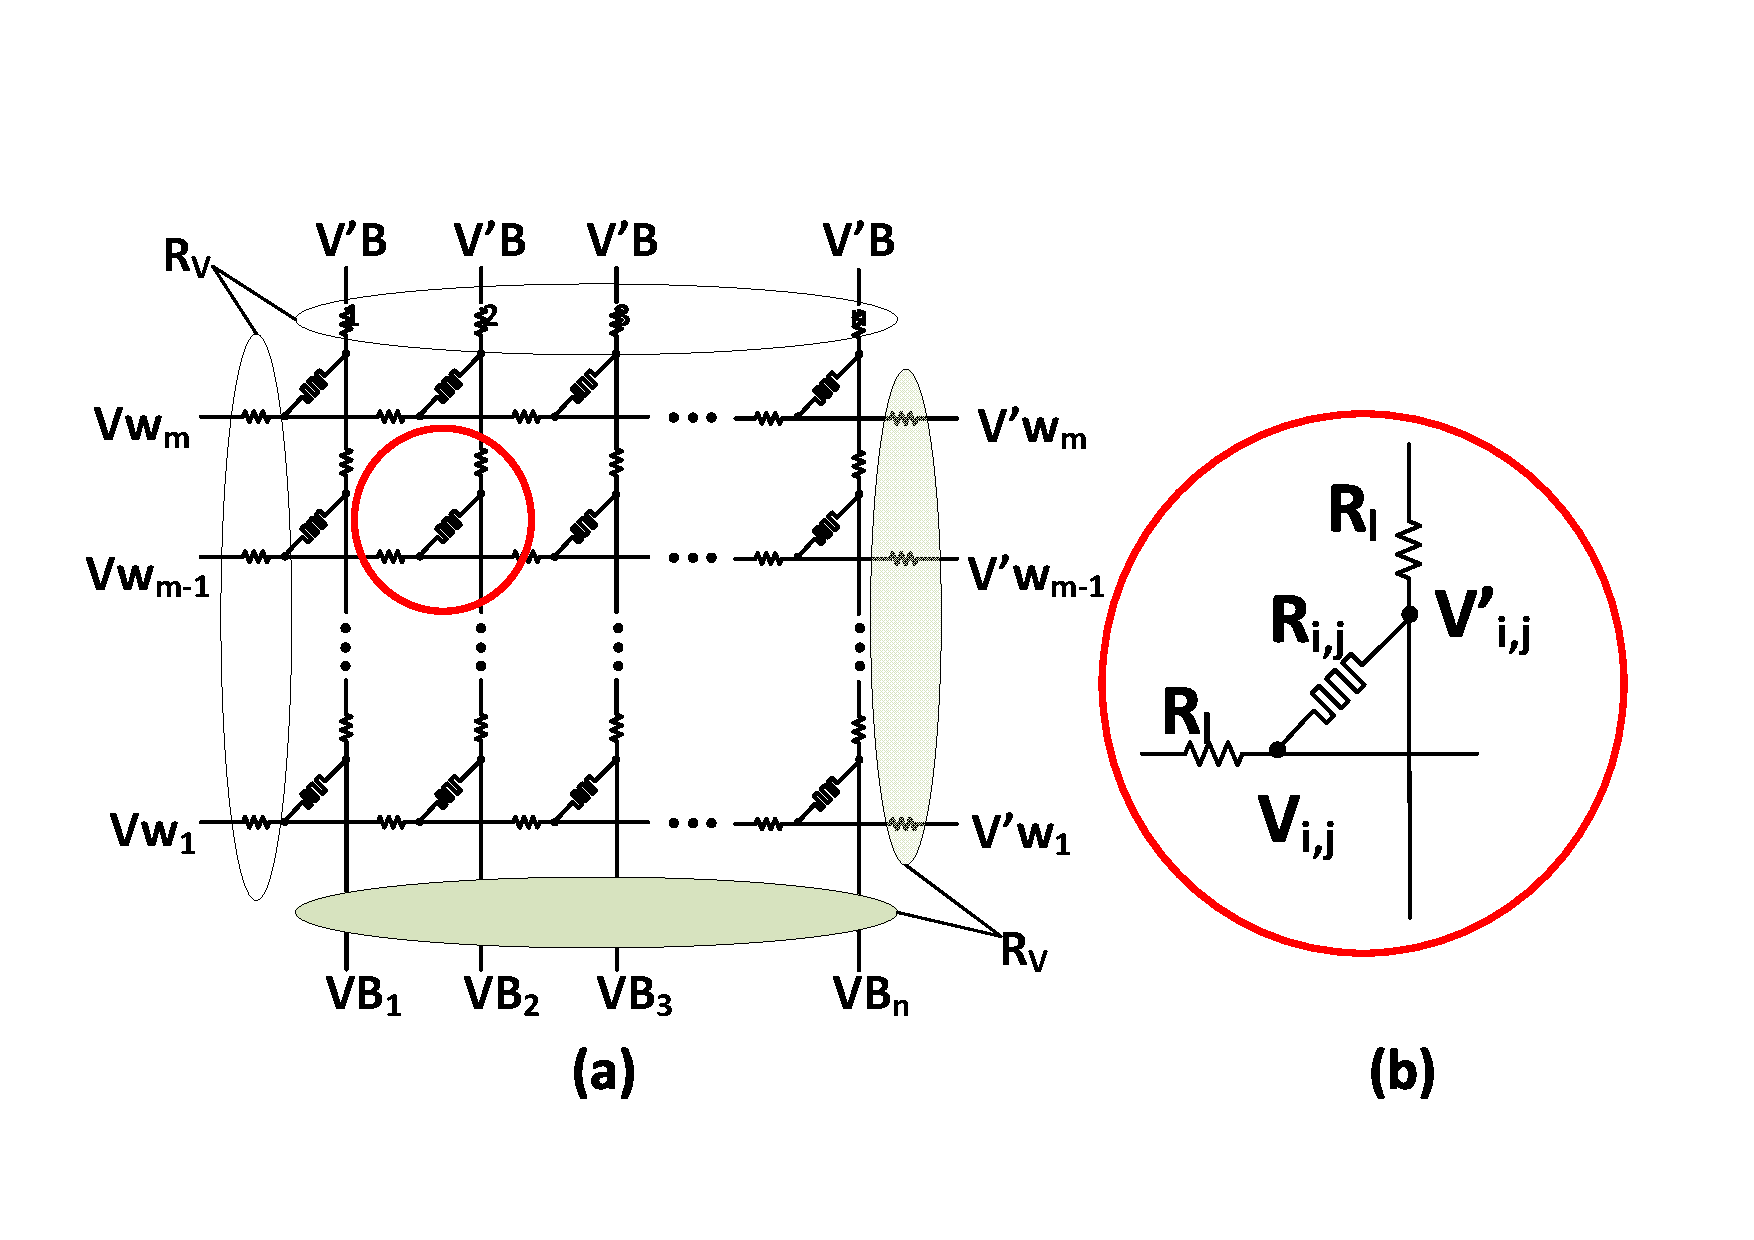
\includegraphics[width=0.45\textwidth]{./figures/model_f.pdf}\\
  \caption{The circuit model of the cross-point array.}\label{fig:modeling}
  \vspace{-12pt}
\end{figure}

%\subsection{Mathematical Model of a Cross-Point Array}
Based on this model, the current equations for each cross-point can be
obtained. All of the cross-points have similar structure with no more than
three current branches, and therefore it is very easy to set up the KCL
equations for each cross-point.

However, it is important to note that KCL equations for cross-points at
the edges of the array vary with different write/read schemes. For
example, the unselected wordline for write operation can be either half
biased or left floating. Thus, the edge conditions should be adjusted
according to each write/read scheme. In particular, according to their
locations and write/read schemes, all of the cross-points in an array can
be classified into three major categories: \emph{normal point},
\emph{activated point} and \emph{floating point}. The normal points are
located inside the memory array. The activated point and floating point
represent the nodes at the edge of cross-point array with different
conditions: an edge point, which is directly connected to the voltage
input or to the ground, can be considered as an activated point.
Otherwise, it is a floating point. The detailed models for these points
can be found in the Appendix. All of the KCL equations can be considered as a system of linear equations, which has the following form
\begin{equation}\label{equ:matrix}
A\cdot V = C,
\end{equation}
where $A$ is a ${2mn\times{2mn}}$ coefficient matrix and $C$ is a
${2mn\times{1}}$ vector, containing the constant terms of these equations.
We demonstrate that all of the KCL equations have simple and similar
structures. Therefore, the linear equation system has a relatively fixed
format and simple structure, making it easy to establish and adjust the
coefficients and constants according to different design schemes. Besides,
due to the simplicity of the KCL equation, $A$ is populated primarily with
zeros and can be saved as a sparse matrix, which will further reduce the
storage cost during the computation.

To validate our analytical model, we compare the results with
HSPICE~\cite{HSPICE} simulations using a resistor model in cross-point
memory arrays. DC analysis was performed by HSPICE which solved the
voltage of every node in the array. The results of eight cross-point
arrays with different array sizes and specific data patterns are shown in
Figure~\ref{fig:validation}, which shows that the voltage drop on the
selected cell derived from our analytical model are consistent with the
HSPICE simulation results.
\begin{figure}%[!t]
\centering\label{fig:SPICE}
  % Requires \usepackage{graphicx}
  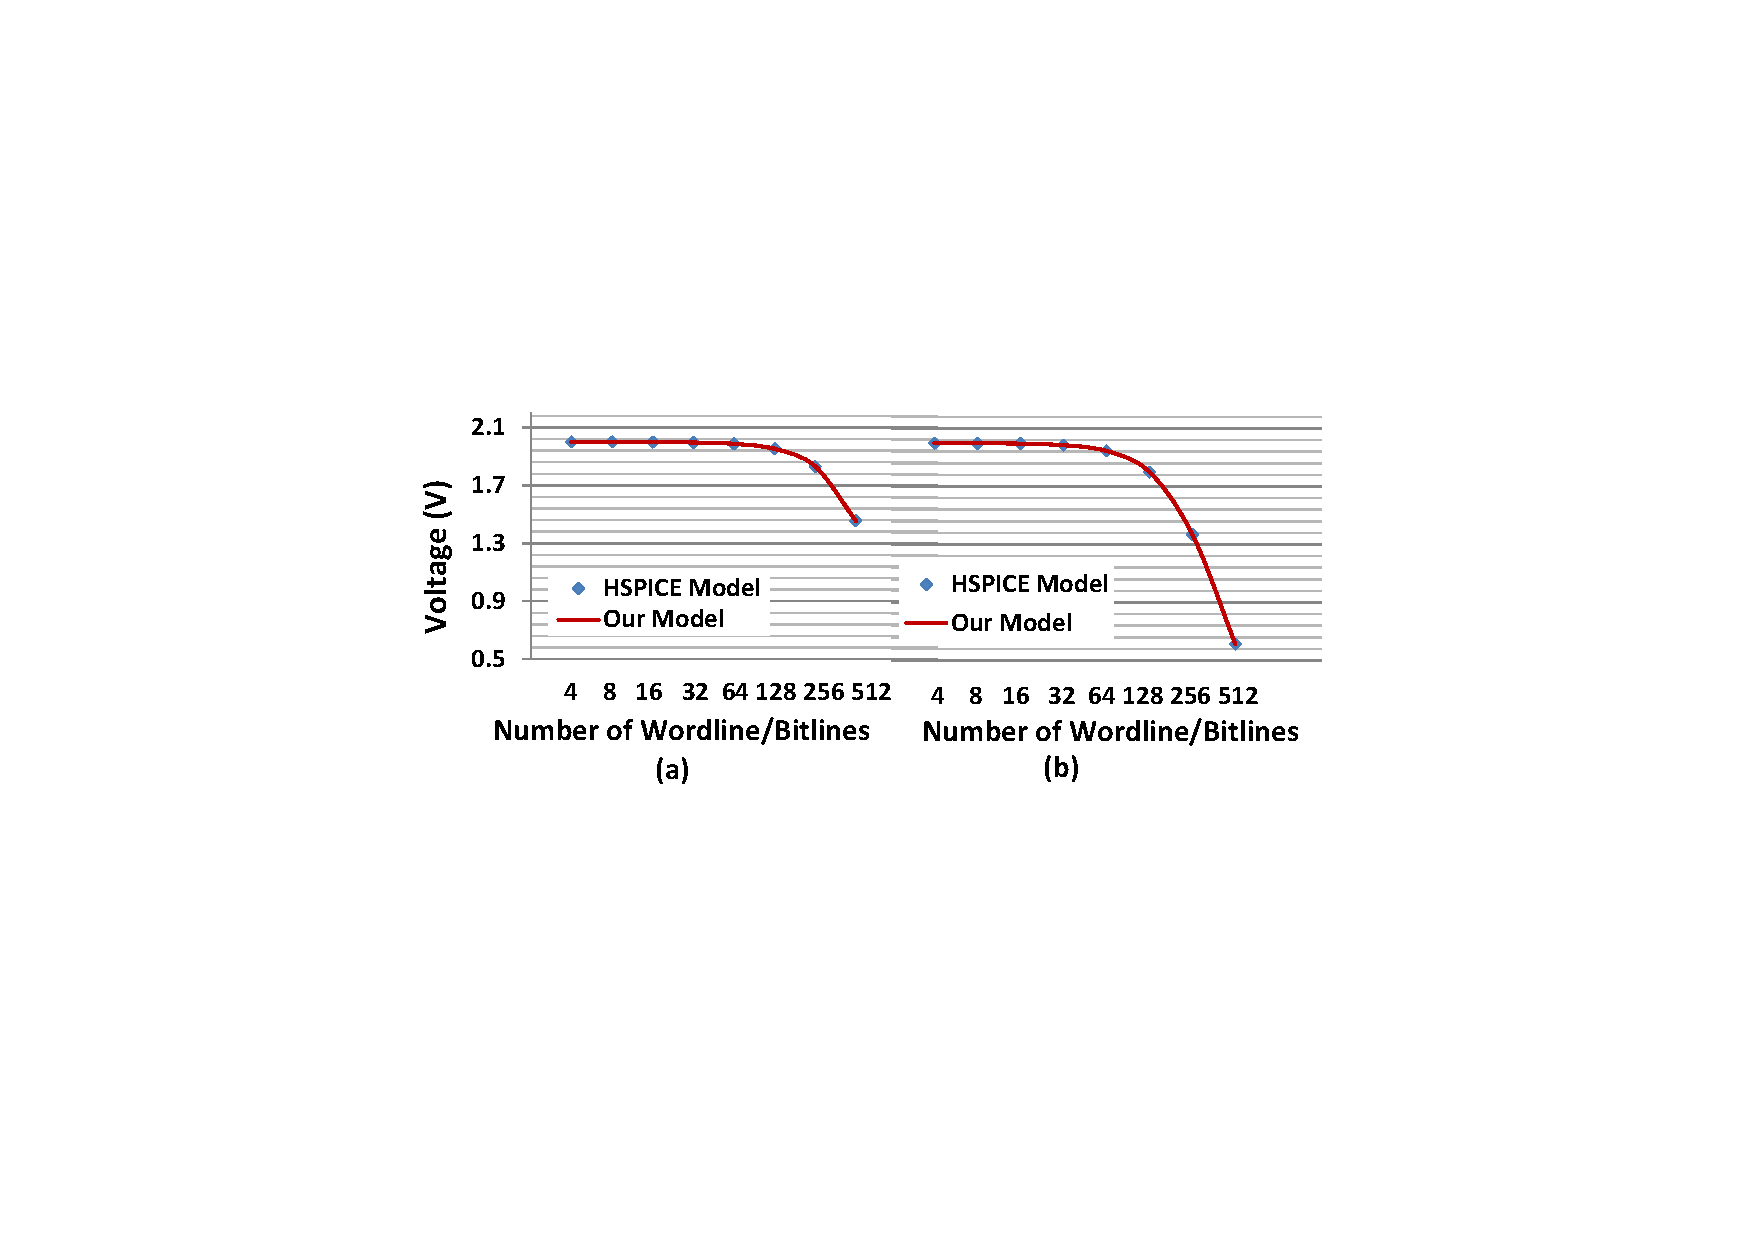
\includegraphics[width=0.5\textwidth]{./figures/SPICE1.pdf}\\
  \caption{Validation of the analytical model against SPICE simulation. The two figures show the voltage drops obtained from our model and SPICE (a) with a nonlinearity factor of 5 and (b) without nonlinearity.}\label{fig:validation}
    \vspace{-10pt}
\end{figure}
%
%The characteristics of the linear system can be summarized as:
%\begin{enumerate}
%  \item
%  As shown in Equation~(\ref{equ:blockedmatrix}), the coefficient matrix $A$ can be further partitioned into 4 smaller subblocks :
%    \begin{equation}\label{equ:blockedmatrix}
%        \mathbf{A} = \left[
%        \begin{array}{cc}
%            A1 & A2  \\
%            A3 & A4  \\
%        \end{array} \right].
%    \end{equation}
%All of these subblocks have the same size of $m\times n$. Subblock
%$A2$ and $A3$ are diagonal matrixes and have the value of: $A2_{i,i} =
%A3_{i,i} = R_{i,i}^{-1}$. $A2$ and $A3$ do not change their values
%with different schemes. However, $A1$ and $A4$ are a little more
%complex than $A2$ and $A3$. $A1$ is a tridiagonal matrix and has
%nonzero elements only in the main diagonal, and the first line below
%and above the diagonal. Similarly, $A_4$ is a special tridiagonal
%matrix, which has nonzero elements in the main diagonal, and the
%$n^{th}$ line below and above the diagonal, where $n$ is the number of
%bitline in the cross-point model. The value of the elements in $A1$
%and $A4$ can be easily derived from Equation (\ref{equ:KCL1}) and
%(\ref{equ:KCL2}). However, the edge condition varies with different
%program schemes. Therefore, the coefficients related to the edge
%condition should be set according to the program schemes. Clearly, the
%four edges shown in Figure~\ref{fig:modeling} correspond to different
%coefficients in $A1$ and $A4$. Due to the space limitations, we
%consider the nodes at the left edge of the array as an example. A
%similar procedure can be followed to initiate the coefficients of
%other edge. The coefficients of nodes at the left edge of the array
%($V_{i,1}$) can be set as:
%
%    \begin{equation}
%    A1(k,k) = \left\{
%    \begin{array}{ll}
%    -(R_l^{-1}+R_{i,1}^{-1})   & \text{if } floating\\
%    -(R_v^{-1}+R_l^{-1}+R_{i,1}^{-1})& \text{if } activated
%    \end{array} \right.
%    \end{equation}
%    where $k=(n-1)i+1$ for $i=1,2...m$.
%
%  \item The constant terms $C$ is a $2mn{\times}1$ vector. Equation(\ref{equ:KCL1})-(\ref{equ:KCL4}) show that only KCL equations of the activated points have constant terms. Therefore, only the following elements in $C$ may have non-zero value: $C((i-1)n+1)$, $C(in)$, $C(mn+i)$ and $C((2m-1)n+i)$ for $i=1,2...m$, corresponding to the nodes at the four edges respectively. Likewise, as an example, we consider nodes $V_{i,1}$. The constant corresponding to these nodes can be defined as:
%    \begin{equation}
%    C((i-1)n+1) = \left\{
%    \begin{array}{ll}
%    0   & \text{if } floating\\
%    -R_v^{-1}V_{Wi}& \text{if } activated
%    \end{array} \right.
%    \end{equation}
%\end{enumerate}
Thus, with parameters such as the resistance of ReRAM cells, the
resistance of interconnect wires, program voltages, and write/read
schemes, voltages at various cross points can be obtained by solving the
system of linear equations. With detailed voltage values,
$V_{2mn{\times}1}$, we can analyze the array at a fine granularity. These
values are also critical to evaluate the reliability, energy consumption,
drive current density, and area overheads of a cross-point array.
